\chapter{Orbite periodiche}
Lo studio delle orbite periodiche si riduce a capire se ci sono ed eventualmente trovarle esplicitamente.

\section{Criteri di non esistenza differenziali}
Intuitivamente se aumento o diminuisco l'area di una regione con il flusso, non posso avere orbite periodiche, perch\'e altrimenti l'area dentro l'orbita si manterrebbe.
\begin{proposition}[Metodo di Bendixon-Dulec]\label{MetodoBendixonDulec}
Consideriamo il sistema $(\dot x,\dot y)=F(x,y)=(f(x,y),g(x,y))$ con $F\in C^1$. Sia $U\subseteq \R^2$ semplicemente connesso e aperto. Se esiste $h:U\to \R^2$ di classe $C^1$ tale che
\[div(h F)(x,y)=\pa{\pp x{h f}+\pp y{hg}}(x,y)\]
ha segno costante in $U$ allora non esistono orbite periodiche interamente contenute in $U$.
\end{proposition}
\begin{proof}
Sia per assurdo $\Gamma$ un orbita periodica contenuta in $U$ e sia $\gamma(t)=(x(t),y(t))$ la sua parametrizzazione con $t\in[0,T]$. Indichiamo con $\wt U\subseteq U$ la componente connessa di $\R^2$ limitata racchiusa da $\Gamma$. Senza perdita di generalit\`a per il segno della divergenza
\begin{align*}
0<&\iint_{\wt U}div(hF)(x,y)dxdy=\\
=&\iint_{\wt U}\pa{\pp x{}(hf)+\pp y{}(hg)dxdy}\pasgnl={(G.G.)}\\
=&\int_{\Gamma^+}hfdy-hgdx=\\
=&\pm\int_0^Th(x(t),y(t))(f(x(t),y(t))\dot y(t)-g(x(t),y(t))\dot x(t))dt\pasgnlmath={(\dot x,\dot y)=(f,g)}0,
\end{align*}
e questo mostra l'assurdo.
\end{proof}

\begin{proposition}[Criterio con gradiente per inesistenza delle orbite periodiche]\label{CriterioGradienteInesistenzaOrbitePeriodiche}
Se $\dot x=F(x)$ con $F$ di classe $C^1$ (anche in $\R^d$) e $F=\nabla I$ allora non esistono orbite periodiche.
\end{proposition}
\begin{proof}
Supponiamo che esista $\Gamma\subseteq U$ orbita periodica e sia $\gamma(t)$ con $t\in [0,T]$ una curva che la parametrizza. Troviamo un assurdo svolgendo il seguente conto
\begin{align*}
0=&I(\gamma(T))-I(\gamma(0))=\int_0^T \dd t{}\pa{I(\gamma(t))}dt=\\
=&\int_0^T \nabla I(\gamma(t))\cdot \dot \gamma(t) dt\pasgnl={$\gamma$ \`e orbita e $\nabla I=F$}\\
=&\int_0^T F(\gamma(t))\cdot F(\gamma(t)) dt=\\
=&\int_0^T \under{\neq 0}{\norm{F(\gamma(t))}^2} dt>0
\end{align*}
dove $F(\gamma(t))\neq \ul0$ perch\'e l'orbita \`e periodica (e quindi non contiene punti fissi).
\end{proof}

\noindent Formalizziamo ora l'idea che se il campo non ruota (o equivalentemente, se il campo \`e conservativo) allora non abbiamo orbite periodiche (se torno al punto di partenza il campo non compie lavoro)
\begin{proposition}[Metodo del rotore]\label{MetodoRotore}
Consideriamo il sistema $(\dot x,\dot y)=F(x,y)=(f(x,y),g(x,y))$ con $F\in C^1$. Se $\pp yf=\pp xg$ su $U$ aperto semplicemente connesso allora non esistono orbite periodiche interamente contenute in $U$.
\end{proposition}
\begin{proof}
Consideriamo $\omega=f dx+gdy$. Per ipotesi, su $U$ vale
\[d\omega=\pa{-\pp yf+\pp xg}dx\wedge dy=0,\]
cio\`e $\omega$ \`e chiusa su $U$. Poich\'e $U$ \`e semplicemente connesso si ha che $\omega$ \`e esatta, dunque esiste $I:U\to \R$ di classe $C^2$ tale che $\omega=dI$, cio\`e $F=\nabla I$. Questo conclude per la proposizione precedente.
\end{proof}


\section{Teoria dell'indice di Poicar\'e nel piano}
Consideriamo sistemi della forma
\[\begin{cases}
\dot x=f(x,y)\\
\dot y=g(x,y)
\end{cases}\]

\begin{definition}[Indice di una curva]
Sia $\Gamma$ una curva chiusa in $\R^2$ regolare (a tratti) \textit{semplice}\footnote{la condizione di semplicit\`a serve per evitare che tutto venga contato con arbitrarie molteplicit\`a.} che non contiene punti fissi. Chiamiamo \textbf{indice di $\Gamma$}
\[I(\Gamma)=\frac1{2\pi}\int_{\Gamma^+}\frac{fdg-gdf}{f^2+g^2}.\]
\end{definition}
\begin{remark}
Quando $f\neq 0$ osserviamo che
\[\frac{fdg-gdf}{f^2+g^2}=d\pa{\arctan\pa{\frac gf}},\]
quindi stiamo contando quante volte $F$ gira seguendo $\Gamma$ in senso diretto. Pi\`u precisamente
\[I(\Gamma)=\#\cpa{\text{giri di $F$ lungo $\Gamma$ in senso antiorario}}-\#\cpa{\text{giri di $F$ in senso orario}}\]
\end{remark}


\setlength{\leftmargini}{0.5cm}
\begin{proposition}[Propriet\`a dell'indice]\label{ProprietaIndice}
Valgono le seguenti affermazioni
\begin{itemize}
\item Sia $H:[0,1]^2\to \R^2, (s,t)\mapsto \gamma_s(t)$ una famiglia continua di curve chiuse regolari a tratti che non contengono punti fissi (le curve sono $\imm\gamma_s=\Gamma_s$). Allora $I(\Gamma_s)$ \`e costante in $s$.
\item Siano $\Gamma_1$ e $\Gamma_2$ curve chiuse regolari a tratti che non contengono punti fissi tali che $\Gamma_1\cap \Gamma_2\neq \emptyset$ ma le regioni da loro racchiuse si intersecano nel vuoto\footnote{per regione racchiusa intendiamo la componente connessa di $\R^2\bs \Gamma$ limitata}, allora
\[I(\Gamma_1+\Gamma_2)=I(\Gamma_1)+I(\Gamma_2),\]
dove $\Gamma_1+\Gamma_2$ \`e la curva dove vengono percorse in successione le due e i tratti in comune vergono percorsi una volta in un senso e una volta nel senso opposto\footnote{Pensa alla somma di $1$-cicli singolari}.
\end{itemize}
\end{proposition}
\begin{proof}
Vedi Geometria 2.
\end{proof}

\begin{definition}[Indice di un punto fisso]
Sia $(x_0,y_0)$ un punto fisso isolato di $F$. L'\textbf{indice di $(x_0,y_0)$} \`e dato dall'indice di una qualsiasi curva chiusa regolare a tratti semplice che lo racchiude e che non racchiude altri punti fissi.
\end{definition}

\begin{proposition}[Indici di alcuni punti fissi]\label{IndiciDiAlcuniPuntiFissi}
Valgono le seguenti affermazioni:
\begin{itemize}
\item $I(\text{nodo})=I(\text{fuoco})=+1$
\item $I(\text{sella})=-1$
\item Se $\Gamma$ \`e un orbita periodica $I(\Gamma)=+1$
\item Se $\Gamma$ \`e una curva regolare a tratti semplice che racchiude solo punti fissi isolati allora 
\[I(\Gamma)=\sum_{\smat{P\text{ punto fisso}\\ P\text{ racchiuso da }\Gamma}}I(P).\]
\end{itemize}
\end{proposition}
\begin{proof}
Per i primi due punti la tesi segue riportandoci al caso lineare standard tramite il teorema di linearizzazione (\ref{TeoremaHartmanGrobman}).\\
Il terzo punto \`e geometricamente evidente date le possibili forme di orbite periodiche in $\R^2$.\\
Il quarto punto segue dalle propriet\`a dell'indice (\ref{ProprietaIndice})\footnote{Vedi teorema dei residui.}.
\end{proof}

\begin{remark}
Un orbita periodica racchiude necessariamente punti fissi i cui indici sommano a $1$. Per esempio un'orbita periodica non pu\`o racchiudere solo una sella.
\end{remark}

\section{Criteri di esistenza di orbite periodiche}
Per trovare esplicitamente orbite periodiche possiamo provare a passare alle coordinate polari
\[\begin{cases}
\dot x=f(x,y)\\
\dot y=g(x,y)
\end{cases} \longrightarrow \begin{cases}
\displaystyle\dot \rho =\frac{x\dot x+y\dot y}{\rho}\\
\displaystyle\dot\theta=\frac{x\dot y-y\dot x}{\rho^2}
\end{cases}\]
dove nel secondo sistema dobbiamo ricordarci $x=\rho\cos\theta$ e $y=\rho\sin\theta$. Per semplicit\`a scriviamo
\[\begin{cases}
\dot \rho=h(\rho,\theta)\\
\dot \theta=\ell(\rho,\theta)
\end{cases}\]
Un'orbita periodica pu\`o essere della forma particolare $\cpa{\rho=\text{cost.}}$.
\begin{proposition}[Criterio polare esistenza orbita periodica]\label{CriterioPolareEsistenzaOrbitaPeriodica}
Dato un sistema in coordinate polari, se esiste $c>0$ tale che per ogni $\theta$ valgono $h(c,\theta)=0$ e $\ell(c,\theta)\neq0$ allora $\cpa{\rho=c}$ \`e invariante\footnote{e quindi $\cpa{x^2+y^2=c^2}$ \`e periodica}.
\end{proposition}
\begin{proof}
Segue dal criterio sull'invarianza di curve di livello (\ref{CostruzioneInsiemiInvariantiCurveDiLivello}) unito all'assenza di punti fissi.
\end{proof}
\noindent Un problema cruciale di questo risultato \`e che la minima perturbazione annichila le ipotesi.

\subsection{Teorema di Poincar\'e-Bendixon}

\begin{definition}[Sezione locale di data larghezza]
Sia $y\in \R^2$ tale che $F(y)\neq 0$. Se $\ell(y)=\Span(v)+y$ \`e la retta passante per $y$ ortogonale a $F(y)$, fissato un $k\in (0,1)$ definiamo la \textbf{sezione locale di larghezza $k$} per $y$ come\footnote{dati due vettori $v$ e $w$, con $\wh{v,w}$ intendiamo l'angolo minore tra essi nel piano generato da $v$ e $w$}
\[S_k(y)=\text{comp. conn. contenente $y$ di }\cpa{z\in \ell(y)\mid \abs{\sin(\wh{v,F(z)})}>k}.\]
\end{definition}

\begin{lemma}[Rettificazione locale]\label{LemmaRettificazioneLocale}
Dato $y\in\R^2$ tale che $F(y)\neq 0$ consideriamo la parametrizzazione di $\ell(y)$ data da $\gamma(u)=y+uv$ al variare di $u\in\R$.
Affermiamo che esitono $V$ e $U$ intorni di $y$ e $0$ rispettivamente e un diffeomorfismo $\psi:U\to V$ tale che $\psi(s,u)=\phi_s(\gamma(u))$.
\end{lemma}

\begin{definition}[Rettangolo di flusso]
Sia $\psi:U\to V$ un diffeomorfismo di rettificazione locale. Fissiamo $\sigma>0,\ \chi>0$ tali che
\[N_{\sigma,\chi}=\cpa{(s,u)\in \R^2\mid |s|\leq \sigma,\ |u|\leq \chi}\subseteq U.\]
Definiamo il \textbf{rettangolo di flusso} per questa scelta di $\sigma$ e $\chi$ come $\Nc_{\sigma,\chi}=\phi(N_{\sigma,\chi})$.
\end{definition}

\begin{lemma}
Se $\Nc_{\sigma,\chi}$ \`e un rettangolo di flusso allora $\Nc_{\sigma,\chi}$ \`e un intorno di $y$ tale che per ogni $z\in \Nc_{\sigma,\chi}$ esiste $\ol t(z)\in (-\sigma,\sigma)$ tale che $\phi_{\ol t}(z)\in S_k(y)$.
\end{lemma}

\begin{figure}[!htb]
    \centering
    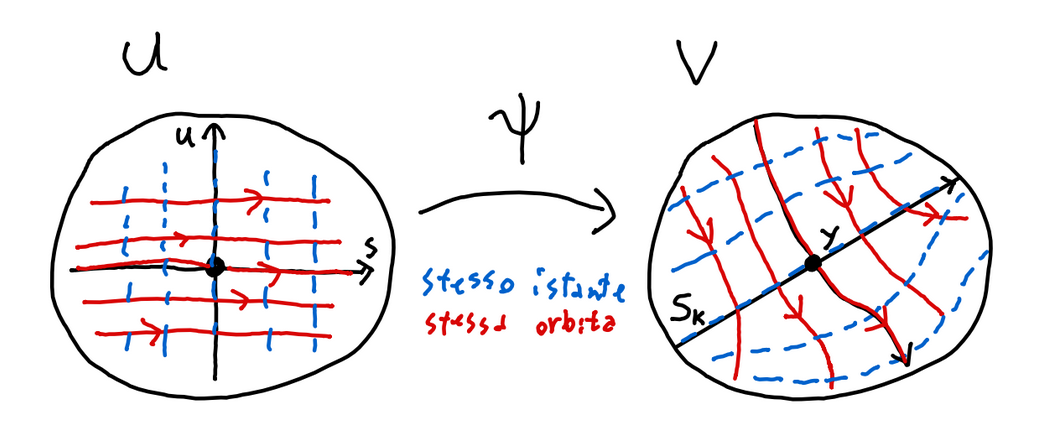
\includegraphics[width=9cm]{Immagini/rettificazione_locale.png}
    \caption{Rappresentazione di come agisce una $\psi$ rettificazione locale come sopra.}
\end{figure}


\begin{theorem}[Poincar\'e-Bendixon]\label{TeoremaPoincareBendixon}
Sia $\dot x=F(x)$ con $F\in C^1(\R^2)$. Supponiamo che esista $D\subseteq \R^2$ compatto non vuoto che non contiene punti fissi e per il quale esiste $x_0\in D$ tale che per qualche $t_0>0$ abbiamo $\phi_t(x_0)\in D$ per ogni $t\geq t_0$.\\
Allora $\Gamma=\omega(x_0)\subseteq D$ \`e un'orbita periodica.
\end{theorem}
\begin{proof}
Sia $x_0\in \R^2$ per cui esiste $t_0>0$ tale che $\phi_t(x_0)\in D$ per ogni $t\geq t_0$. Allora $\omega(x_0)$ \`e non vuoto, invariante e $\omega(x_0)\subseteq D$ per (\ref{OrbitaPositivaLimitataImplicaCompattezzaEInvarianzaOmegaLimite}). Scelto $x\in \omega(x_0)\subseteq D$ allora $\Oc^+(x)\subseteq \omega(x_0)$ e quindi $\omega(x)\subseteq \omega(x_0)$. Sia $y\in \omega(x)$
\vspace{0.25cm}

\noindent
\ul{Claim:} $\#(S_k(y)\cap \Oc^+(x))=1$.
\begin{proof}[Dimostrazione del claim]
Mostriamo prima che l'intersezione \`e non vuota e poi mostriamo che contiene un'unico punto.
\setlength{\leftmargini}{0cm}
\begin{itemize}
\item[$\boxed{\neq \emptyset}$] Per definizione di $\omega(x)$ esiste una successione monotona $t_k\nearrow +\infty$ tale che $\phi_{t_k}(x)\to y$. Poich\'e $\Nc_{\sigma,\chi}$ \`e un intorno di $y$, per definizione di convergenza esiste $\ol t>\sigma$ tale che $\phi_{\ol t}(x)\in \Nc_{\sigma,\chi}$. Per il lemma precedente esiste allora $\wh t\in (-\sigma,\sigma)$ tale che $\phi_{\wh t}(\phi_{\ol t}(x))\in S_k(y)$. Ponendo $\wh t+\ol t=\wt t$ esiste $\wt t>0$ tale che $\phi_{\wt t}(x)\in S_k(y)$.
\item[$\boxed{\#=1}$] Supponiamo per assurdo che esistano $x_1,x_2\in S_k(y)\cap \Oc^+(x)\subseteq \omega(x_0)$ distinti. Per definizione di $\omega$-limite esistono $\tau_{j}^1\nearrow+\infty$ e $\tau_{j}^2\nearrow+\infty$ tali che 
\[\lim_{j\to+\infty}\phi_{\tau^1_j}(x_0)=x_1,\quad \lim_{j\to+\infty}\phi_{\tau^2_j}(x_0)=x_2.\]
Esistono dunque per il lemma $\wt \tau^1_j$ e $\wt \tau^2_j$ tali che $\phi_{\wt \tau^i_j}(x_0)\in S_k(y)$. Siano $U_1$ e $U_2$ intorni di $x_1$ e $x_2$ disgiunti. Per $j$ abbastanza grande abbiamo che $\phi_{\wt \tau^i_j}(x_0)\in U_i$.\\
Poich\'e sia $\wt \tau_j^1$ che $\wt \tau_j^2$ vanno a $+\infty$, esistono $\xi_1<\xi_2<\xi_3$ tali che
\[\phi_{\xi_1}(x_0)\in U_1,\ \phi_{\xi_2}(x_0)\in U_2,\ \phi_{\xi_3}(x_0)\in U_1.\]
Sia $\wt \Gamma$ la curva chiusa data da
\[\wt \Gamma=\cpa{\al\phi_{\xi_1}(x_0)+(1-\al)\phi_{\xi_2}(x_0)\mid \al\in [0,1]}\cup \bigcup_{s\in (\xi_1,\xi_2)}\phi_s(x_0).\]
Per definizione di $S_k(y)$ e per unicit\`a locale si ha che $\Oc^+(\phi_{\xi_2}(x_0))$ \`e contenuto nella componente connessa limitata definita da $\wt \Gamma$, ma questo \`e assurdo perch\'e esiste $\Delta t=\xi_3-\xi_2$ \`e tale che $\phi_{\Delta t}(\phi_{\xi_2}(x_0))=\phi_{\xi_3}(x_0)$ ma per definizione di $S_k(y)$ un'orbita che parte da $S_k(y)$ torna a $S_k(y)$ dal lato opposto rispetto a quello di partenza.
\begin{figure}[!htb]
    \centering
    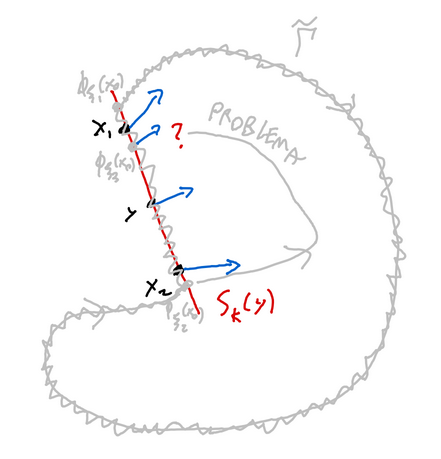
\includegraphics[width=5cm]{Immagini/poincare_bendixon.png}
    \caption{Rappresentazione grafica dell'assurdo trovato.}
\end{figure}

\end{itemize}
\setlength{\leftmargini}{0.5cm}
\end{proof}
\noindent
Sia $y\in \omega(x)$ e sia $\wt t>0$ tale che $\phi_{\wt t}(x)\in S_k(y)$ (esiste per il primo punto del claim). Sappiamo che esiste $\tau>\wt t$ tale che $\phi_{\tau}(x)\in \Nc_{\sigma,\chi}$ (convergenza di successioni). Esiste dunque $\wt \tau\in (-\sigma,\sigma)$ tale che $\phi_{\tau+\wt \tau}(x)\in S_k(y)$ (lemma) e per il secondo punto del claim $\phi_{\tau+\wt\tau}(x)=\phi_{\wt t}(x)$, dunque $\Gamma=\Oc(x)$ \`e periodica.
\vspace{0.25cm}

\noindent
Osserviamo che $\Gamma\subseteq \omega(x_0)$ per costruzione. L'altro contenimento segue come segue:\\
Per definizione $x=\lim_j\phi_{t_j}(x_0)$. Se $z=\phi_{s}(x)$ allora per continuit\`a del flusso $z=\lim_j\phi_{t_j+s}(x_0)$.
\end{proof}

\begin{remark}
Osserviamo che $D$ come nel teorema di Poicar\'e-Bendixon non pu\`o essere semplicemente connesso per la teoria dell'indice.
\end{remark}

\begin{fact}[Poincar\'e-Bendixon generale]
Se per $x_0$ esiste $t_0>0$ tale che $\phi_t(x_0)\in D$ per ogni $t\geq t_0$ con $D$ non vuoto e compatto allora $\omega(x_0)$ pu\`o essere
\begin{itemize}
\item punto fisso
\item orbita periodica
\item unione di punti fissi e orbite eterocline
\item punto fisso e orbita omoclina
\end{itemize}
\end{fact}

\begin{example}
Consideriamo il sistema
\[\begin{cases}
\dot \rho=\rho(1-\rho^2) + \e f(x,y)\\
\dot \theta=1+\e g(x,y)
\end{cases}\]
Se $f,g\in C^1$ allora esiste $\e_0>0$ tale che per ogni $\e<\e_0$ esiste un orbita periodica.\\
Proviamo a definire
\[D=\cpa{\rho_1\leq\rho\leq\rho_2}\]
Osserviamo che nel caso non perturbato, per $\rho<1$ allora $\dot \rho>0$ mentre per $\rho>1$ allora $\dot \rho<0$.\\
Sia $M=\max\cpa{\norm {f\res{\cpa{\rho\leq 5}}}_\infty, \norm {g\res{\cpa{\rho\leq 5}}}_\infty}$ (dove $5$ \`e un qualche valore ``grosso"). Proviamo a definire $D=\cpa{\frac12\leq \rho\leq 2}$.\\
$\rbar{\dot \rho}_{\rho=\frac12}=\frac38+\e f(\frac12,\theta)\geq \frac38-\e M$ e questo \`e maggiore di $0$ per $\e<\frac3{8M}$.
Similmente per $\rbar{\dot \rho}_{\rho=2}$ chiediamo $\e<\frac6M$. Cerchiamo allora stime tali che
$\rbar{\dot \theta}_{\cpa{\frac12\leq \rho\leq 2}}\neq 0$ e dopo conti simili troviamo che $\e_0=\frac3{8M}$ rispetta tutte le condizioni volute.
\end{example}